\section{Comportamiento}
\label{seccion-comportamiento-apis}
Para comprender el comportamiento de las APIs de alto nivel, es necesario complementar lo detallado sobre la clase OpenGlove en la Subsección \ref{subseccion-estructura-apis-hl}, en la cual se habló sobre la estructura de las mismas. Cada instancia de la clase OpenGlove de alto nivel, permite ejecutar acciones sobre su cliente WebSocket, el servidor WebSocket al que se conecta, a las configuraciones de su instancia de la clase OpenGloveDevice alojada en el servidor y realizar acciones sobre el software de control Arduino. Además, cada instancia provee un fácil consumo de los datos provenientes de Arduino. La suma de esto es lo que hace posible una representación de los dispositivos OpenGlove en las APIs de alto nivel en tiempo real, incluyendo el envío de mensajes de manera bidireccional y full-duplex para los lenguajes de programación C\# y Java. Con esto se facilita que otras APIs de alto nivel pueden ser desarrolladas, utilizando lenguajes de programación que permitan: el manejo de eventos o funciones lambda o el envío de mensajes entre hilos, además del uso de Clientes WebSocket (API WebSocket y protocolo RFC 6455). De esta forma, se reduce la necesidad de agregar lógica compleja en la API de alto nivel.

A continuación se describe el comportamiento general de los métodos disponibles en las APIs de alto nivel, utilizando diagramas de actividades. Se agruparon estos métodos según su nivel de interacción con las diferentes capas de abstracción del SDK. Las capas de abstracción corresponden a: la API de alto nivel (Cliente WebSocket), el Servidor WebSocket, las instancias de la clase OpenGloveDevice, las instancias de LegacyOpenGlove (API C\# de bajo nivel) y el software de control Arduino.



\subsection{Métodos aplicados sobre cliente WebSocket}
\label{subsection:method-websocket-client}

Los métodos que pueden ser aplicados sobre el cliente WebSocket se muestran en la Figura \ref{fig:methods-0-api-hl}. Estos métodos son ejecutados por la aplicación que utiliza una instancia de OpenGlove, realizando la acción sobre el cliente WebSocket. Esto se detalla en el diagrama de actividades de la Figura \ref{fig:activity-diagrams-0-api-hl}. Adicionalmente, en el caso que se logre la conexión con el servidor WebSocket, el evento OnOpen del cliente es invocado. Cuando se invoca ese evento, se agrega la instancia OpenGlove al servidor  y se inicia la captura de datos. Eso se realizó utilizando los métodos AddOpenGloveDeviceToServer y StartCaptureDataFromServer respectivamente. El comportamiento de estos dos métodos mencionados se incluyen en la Subsección \ref{subsection:method-websocket-server}.

\begin{figure}[H]
  \begin{center} 
      \begin{lstlisting}
	// OpenGloveActions: OpenGlove High level API (WebSocketClient)
	public void ConnectToWebSocketServer();
	public void DisconnectFromWebSocketServer();
	\end{lstlisting}
   \captionsetup{justification=centering}
    \caption[Métodos aplicados sobre el cliente WebSocket]{Métodos aplicados sobre el cliente WebSocket \\Fuente: Elaboración propia (2018)}
    \label{fig:methods-0-api-hl}
  \end{center}
\end{figure}



\begin{figure}[H]
  \begin{center} 
   	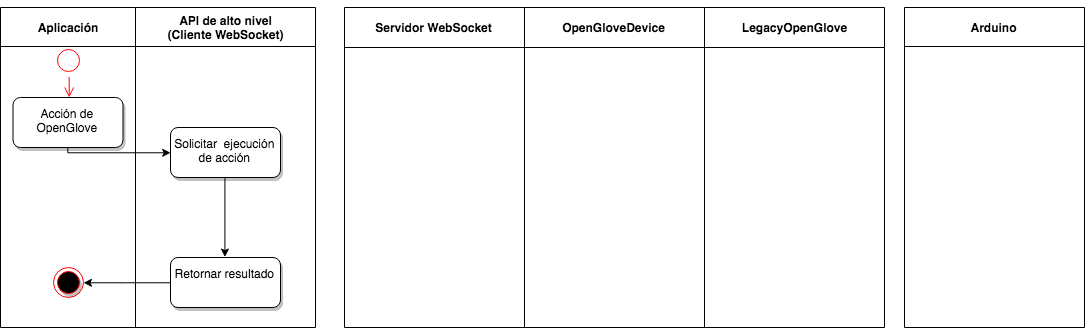
\includegraphics[width=1.0\textwidth]{images/chapter04/ActivityDiagrams-OpenGloveActions-0.png} 
   	\captionsetup{justification=centering}
    \caption[Diagrama de actividades de los métodos aplicados sobre el cliente WebSocket]{Diagrama de actividades de los métodos aplicados sobre el cliente WebSocket\\Fuente: Elaboración propia (2018)}
    \label{fig:activity-diagrams-0-api-hl}
  \end{center}
\end{figure}




\subsection{Métodos aplicados sobre servidor WebSocket}
\label{subsection:method-websocket-server}
Los métodos que pueden ser aplicados sobre el servidor WebSocket se muestran en la Figura \ref{fig:methods-1-websocket-server}. Estos métodos son ejecutados por la aplicación que utiliza una instancia de OpenGlove, realizando la acción sobre el servidor WebSocket, pasando por la capa intermedia del cliente WebSocket. El comportamiento de estos métodos se aprecia en el diagrama de actividades de la Figura \ref{fig:activity-diagrams-1-websocket-server}.




\begin{figure}[H]
  \begin{center} 
\begin{lstlisting}
// OpenGloveActions: WebSocket Server
public void AddOpenGloveDeviceToServer();
public void RemoveOpenGloveDeviceFromServer();
public void SaveOpenGloveConfiguration();
public void StartCaptureDataFromServer();
public void StopCaptureDataFromServer();
\end{lstlisting}
   \captionsetup{justification=centering}
    \caption[Métodos aplicados sobre el servidor WebSocket]{Métodos aplicados sobre el servidor WebSocket \\Fuente: Elaboración propia (2018)}
    \label{fig:methods-1-websocket-server}
  \end{center}
\end{figure}


\begin{figure}[H]
  \begin{center} 
   	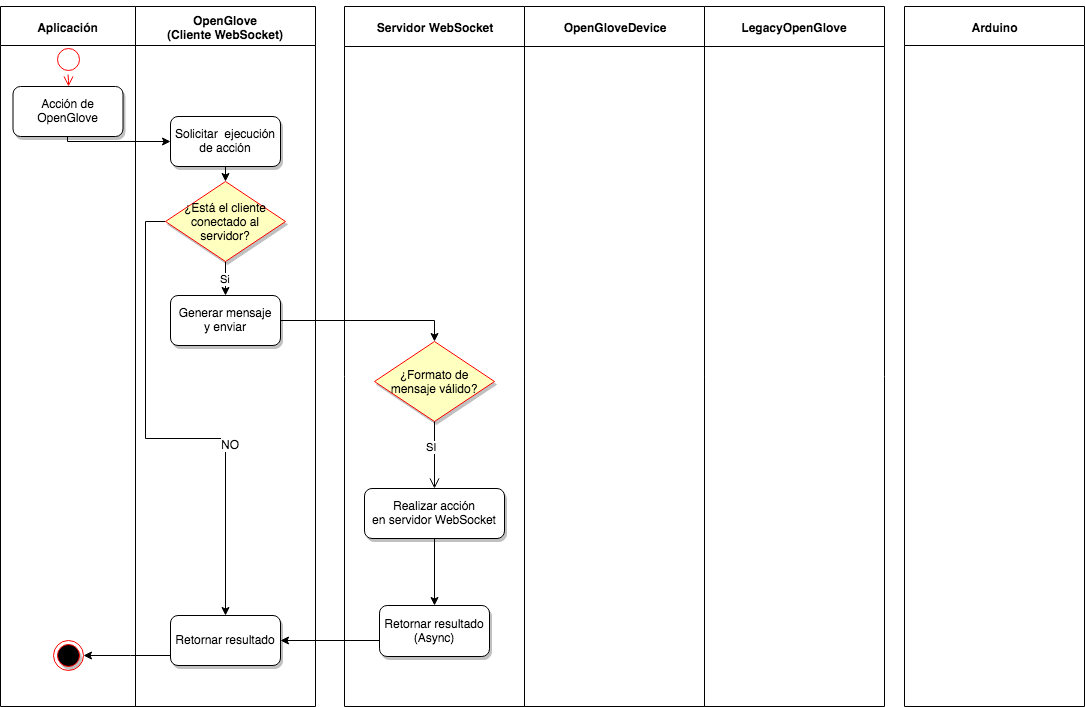
\includegraphics[width=1.0\textwidth]{images/chapter04/ActivityDiagrams-OpenGloveActions-1.png} 
   	\captionsetup{justification=centering}
    \caption[Diagrama de actividad de los métodos aplicados sobre el servidor WebSocket]{Diagrama de actividad de los métodos aplicados sobre el servidor WebSocket\\Fuente: Elaboración propia (2018)}
    \label{fig:activity-diagrams-1-websocket-server}
  \end{center}
\end{figure}





\subsection{Métodos aplicados sobre instancias de OpenGloveDevice}
\label{subsection:method-openglove-device}
Los métodos que pueden ser aplicados sobre la instancia de la clase OpenGloveDevice en el servidor WebSocket se muestran en la Figura \ref{fig:methods-2-openglove-device}. Estos métodos son ejecutados por la aplicación que utiliza una instancia de OpenGlove, realizando la acción sobre la instancia de OpenGloveDevice en el servidor WebSocket, pasando por las capas intermedias del cliente y el servidor WebSocket. El comportamiento de estos métodos se puede apreciar en el diagrama de actividades de la Figura \ref{fig:activity-diagrams-2-openglove-device}.


\begin{figure}[H]
  \begin{center} 
\begin{lstlisting}
// OpenGloveActions: OpenGlove Instances
public void ConnectToBluetoothDevice();
public void DisconnectFromBluetoothDevice();
public void AddActuator(int region, int positivePin, int negativePin);
public void AddActuators(List<int> regions, List<int> positivePins, List<int> negativePins);
public void AddFlexor(int region, int pin);
public void AddFlexors(List<int> regions, List<int> pins);
public void SetThreshold(int value);
public void SetIMUStatus(bool status);
public void SetRawData(bool status);
public void SetIMUChoosingData(int value);
public void SetLoopDelay(int value);
\end{lstlisting}
   	\captionsetup{justification=centering}
    \caption[Métodos aplicados sobre instancias de OpenGloveDevice]{Métodos aplicados sobre instancias de OpenGloveDevice\\Fuente: Elaboración propia (2018)}
    \label{fig:methods-2-openglove-device}
  \end{center}
\end{figure}

\begin{figure}[H]
  \begin{center} 
   	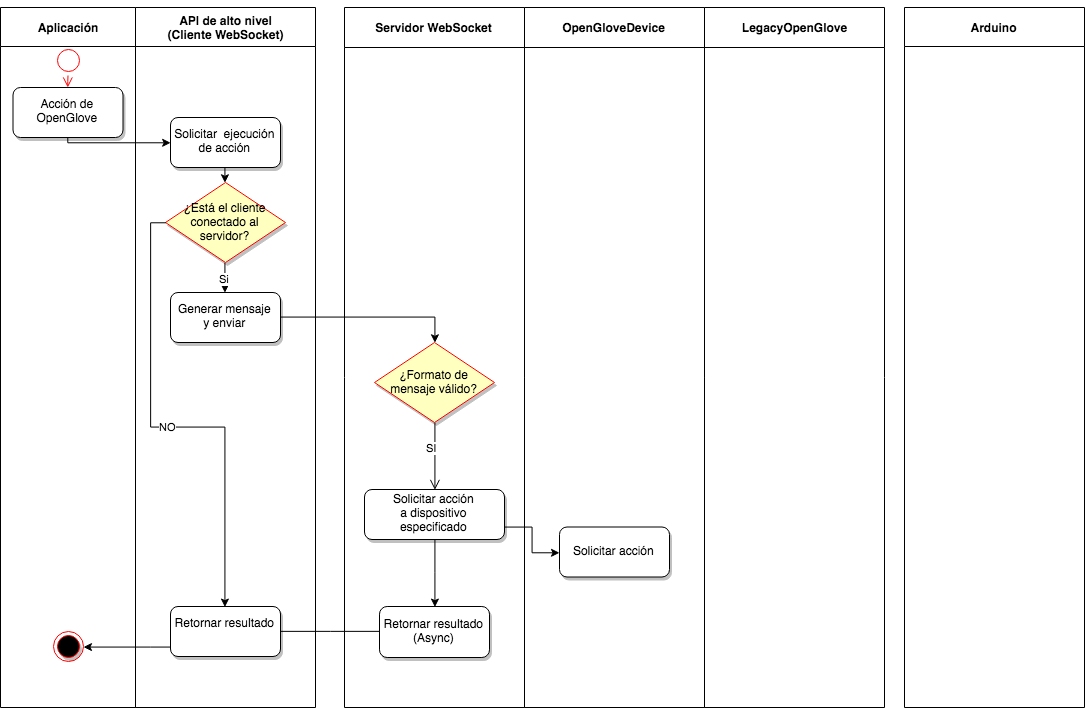
\includegraphics[width=1.0\textwidth]{images/chapter04/ActivityDiagrams-OpenGloveActions-2.png} 
   	\captionsetup{justification=centering}
    \caption[Diagrama de actividades de las acciones OpenGlove sobre instancias de OpenGloveDevice en servidor]{Diagrama de actividades de las acciones OpenGlove sobre instancias de OpenGloveDevice en servidor\\Fuente: Elaboración propia (2018)}
    \label{fig:activity-diagrams-2-openglove-device}
  \end{center}
\end{figure}



\subsection{Métodos aplicados sobre el software de control Arduino}
\label{subsection:method-openglove-arduino}
Los métodos que pueden ser aplicados sobre el software de control Arduino se muestran en la Figura \ref{fig:methods-3-openglove-arduino}. Estos métodos son ejecutados por la aplicación que utiliza una instancia de OpenGlove, realizando la acción sobre el software de control Arduino. Estos métodos generan cambios en el dispositivo Arduino. Para realizar la acción se pasa por las capas intermedias del cliente, el servidor WebSocket y la instancia de OpenGloveDevice que administra la conexión con Arduino. El comportamiento de estos métodos se puede apreciar en el diagrama de actividades de la Figura \ref{fig:activity-diagrams-3-openglove-arduino}.


\begin{figure}[H]
  \begin{center} 
\begin{lstlisting}
// OpenGloveActions: Software of Control Arduino
public void Start();
public void Stop();
public void RemoveActuator(int region);
public void RemoveActuators(List<int> regions);
public void ActivateActuators(List<int> regions, List<string> intensities);
public void ActivateActuatorsTimeTest(List<int> regions, List<string> intensities);
public void TurnOnActuators();
public void TurnOffActuators();
public void TurnOnFlexors();
public void TurnOffFlexors();
public void ResetActuators();
public void RemoveFlexor(int region);
public void RemoveFlexors(List<int> regions);
public void CalibrateFlexors();
public void ConfirmCalibration();
public void ResetFlexors();
public void StartIMU();
public void ReadOnlyAccelerometerFromIMU();
public void ReadOnlyGyroscopeFromIMU();
public void ReadOnlyMagnetometerFromIMU();
public void ReadOnlyAttitudeFromIMU();
public void ReadAllDataFromIMU();
public void TurnOnIMU();
public void TurnOffIMU();
public void GetOpenGloveArduinoVersionSoftware();
\end{lstlisting}
   	\captionsetup{justification=centering}
    \caption[Métodos aplicados sobre el software de control Arduino]{Métodos aplicados sobre el software de control Arduino\\Fuente: Elaboración propia (2018)}
    \label{fig:methods-3-openglove-arduino}
  \end{center}
\end{figure}



\begin{figure}[H]
  \begin{center} 
   	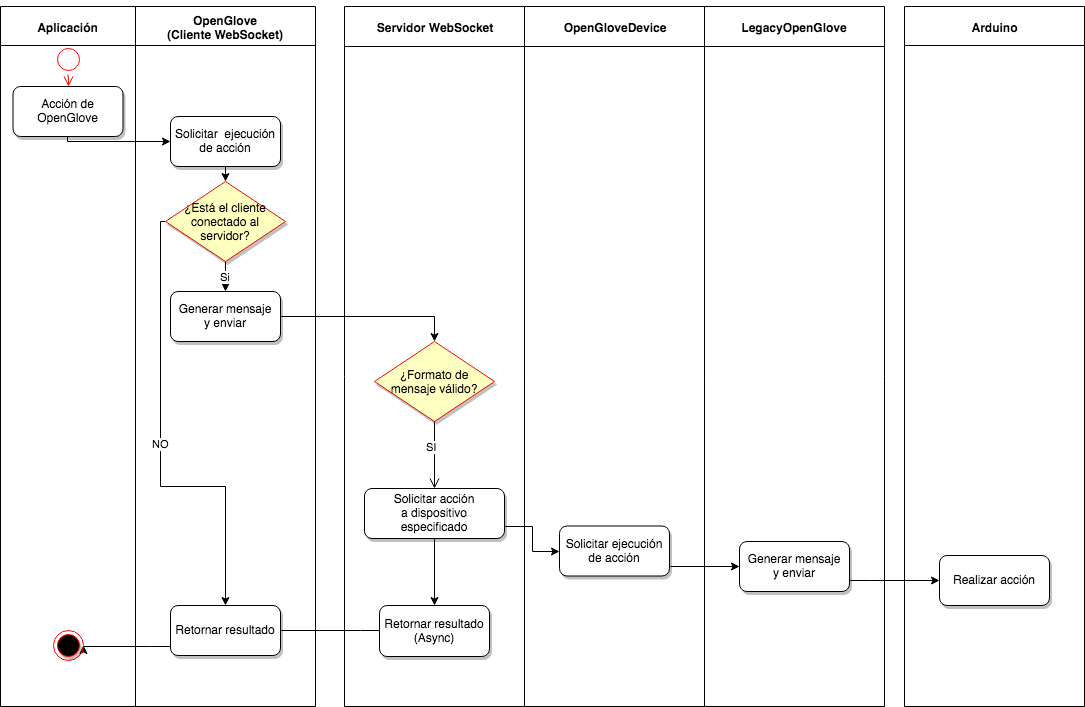
\includegraphics[width=1.0\textwidth]{images/chapter04/ActivityDiagrams-OpenGloveActions-3.png} 
   \captionsetup{justification=centering}
    \caption[Diagrama de actividades de los métodos aplicados sobre el software de control Arduino]{Diagrama de actividades de los métodos aplicados sobre el software de control Arduino\\Fuente: Elaboración propia (2018)}
    \label{fig:activity-diagrams-3-openglove-arduino}
  \end{center}
\end{figure}


\subsection{Escuchando mensajes provenientes de Arduino}
\label{subsection:reading-openglove-arduino}
Este comportamiento ocurre cuando se ha inicializado por lo menos un flexor y/o se ha inicializado e iniciado la IMU. La Figura \ref{fig:methods-4-listening-arduino}, muestra el formato de los métodos que deben ser implementados por los objetos que utilicen instancias de la clase OpenGlove. El comportamiento de estos métodos se aprecia en el Diagrama de actividades de la Figura \ref{fig:activity-diagrams-4-ListeningMessagesFromArduino}

\begin{figure}[H]
  \begin{center}
\begin{lstlisting}
// OpenGloveActions: Listening messages from Arduino Control Software
// For use in API C#: subcribe to event with your own method
// For use in API Java: implements public interface with lambdas or method references
public void OnTimeTestServerLatencyActivateActuatorsReceived(long nanoSeconds);
public void OnTimeTestArduinoLatencyActivateActuatorsReceived(long microSeconds);
public void OnFlexorValueReceived(int region, int value);
public void OnAccelerometerValuesReceived(float ax, float ay, float az);
public void OnGyroscopeValuesReceived(float gx, float gy, float gz);
public void OnMagnometerValuesReceived(float mx, float my, float mz);
public void OnAttitudeValuesReceived(float pitch, float roll, float yaw);
public void OnAllIMUValuesReceived(float ax, float ay, float az, float gx, float gy, float gz, float mx, float my, float mz);
public void OnInfoMessagesReceived(string message);
\end{lstlisting}
   	\captionsetup{justification=centering}
    \caption[Lectura de mensajes provenientes de Arduino]{Lectura de mensajes provenientes de Arduino\\Fuente: Elaboración propia (2018)}
    \label{fig:methods-4-listening-arduino}
  \end{center}
\end{figure}

\begin{figure}[H]
  \begin{center} 
   	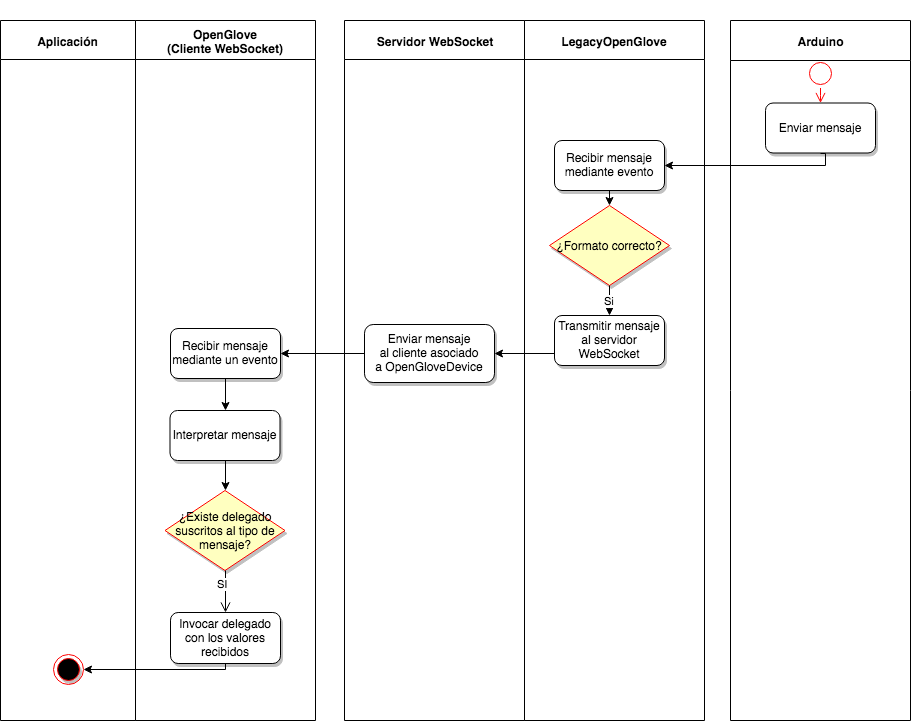
\includegraphics[width=1.0\textwidth]{images/chapter04/ActivityDiagrams-ListeningMessagesFromArduino.png} 
   	\captionsetup{justification=centering}
    \caption[Diagrama de actividades de la lectura de mensajes provenientes de Arduino]{Diagrama de actividades de la lectura de mensajes provenientes de Arduino\\Fuente: Elaboración propia (2018)}
    \label{fig:activity-diagrams-4-ListeningMessagesFromArduino}
  \end{center}
\end{figure}

\subsection{Escuchando el estado de conexión del dispositivo Bluetooth}
\label{subsection:reading-bluetooth-device-state}

Para actualizar el estado de la conexión Bluetooth en las APIs de alto nivel, el hilo que administra dicha conexión, debe enviar  actualizaciones del estado de conexión o desconexión con los dispositivos. Cuando el estado del socket está conectado se envía un mensaje  \textit{``b,True"}  y cuando no, se envía \textit{``b,False"}. La Figura \ref{fig:methods-5-listening-bluetoothdevice-state}, muestra el método que se debe implementar para obtener los cambios de estado de la conexión Bluetooth.  El comportamiento de activación de estos métodos se puede apreciar en el diagrama de actividades de la Figura \ref{fig:activity-diagrams-5-listening-bluetoothdevice-state}.

\begin{figure}[H]
  \begin{center}
\begin{lstlisting}
// OpenGloveActions: Listening Bluetooth device connection state messages
// For use in API C#: subcribe to event with your own method
// For use in API Java: implements public interface with lambdas or method references
public void OnBluetoothDeviceConnectionStateChanged(bool isConnected);
\end{lstlisting}
   	\captionsetup{justification=centering}
    \caption[Lectura del estado de conexión del dispositivo Bluetooth]{Lectura del estado de conexión del dispositivo Bluetooth\\Fuente: Elaboración propia (2018)}
    \label{fig:methods-5-listening-bluetoothdevice-state}
  \end{center}
\end{figure}

\begin{figure}[H]
  \begin{center} 
   	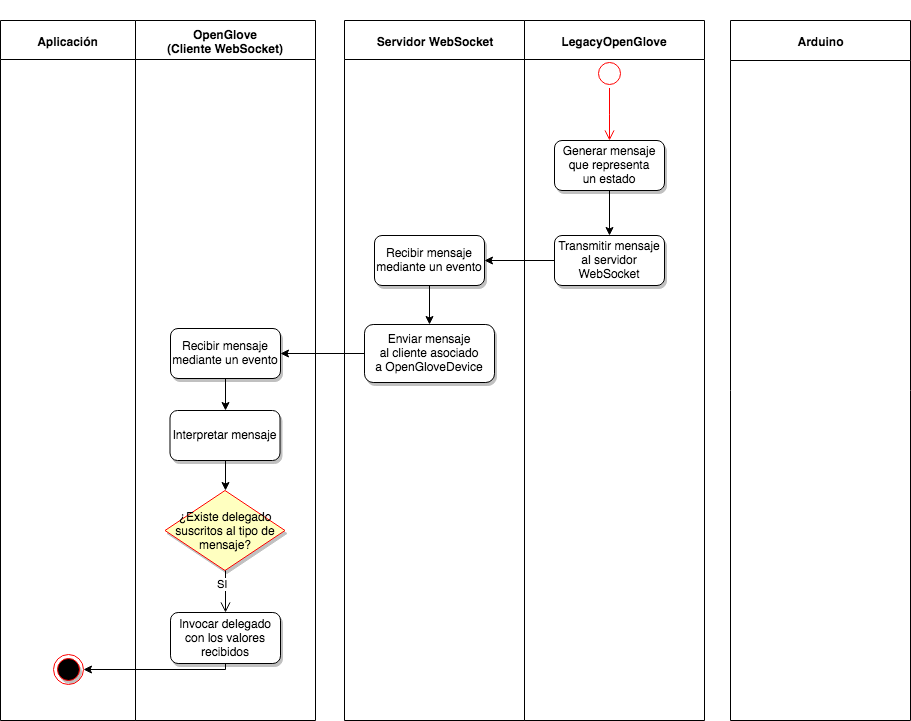
\includegraphics[width=1.0\textwidth]{images/chapter04/ActivityDiagrams-ListeningMessagesFromOpenGloveDevice.png} 
   	\captionsetup{justification=centering}
    \caption[Diagrama de actividades del método que escucha la conexión del dispositivo Bluetooth]{Diagrama de actividades del método que escucha la conexión del dispositivo Bluetooth\\Fuente: Elaboración propia (2018)}
    \label{fig:activity-diagrams-5-listening-bluetoothdevice-state}
  \end{center}
\end{figure}


\subsection{Escuchando el estado de conexión del cliente WebSocket}
\label{subsection:listening-openglove-arduino}
Para notificar el estado de la conexión del cliente WebSocket en las APIs de alto nivel, se invoca el método OnWebSocketConnectionStateChanged, cada vez que ocurre un cambio utilizando OnOpen y OnClose de la API WebSocket. La Figura \ref{fig:methods-6-listening-websocket-state}, muestra el método que debe ser implementado para escuchar el estado de conexión del cliente WebSocket. El comportamiento de este método se puede apreciar en el diagrama de actividades de la Figura \ref{fig:activity-diagrams-6-listening-websocket-state}.


\begin{figure}[H]
  \begin{center}
\begin{lstlisting}
// OpenGloveActions: Listening WebSocket client connection state messages
// For use in API C#: subcribe to event with your own method
// For use in API Java: implements public interface with lambdas or method references
public void OnWebSocketConnectionStateChanged(bool isConnected);
\end{lstlisting}
   	\captionsetup{justification=centering}
    \caption[Lectura del estado de conexión del cliente WebSocket]{Lectura del estado de conexión del cliente WebSocket\\Fuente: Elaboración propia (2018)}
    \label{fig:methods-6-listening-websocket-state}
  \end{center}
\end{figure}


\begin{figure}[H]
  \begin{center} 
   	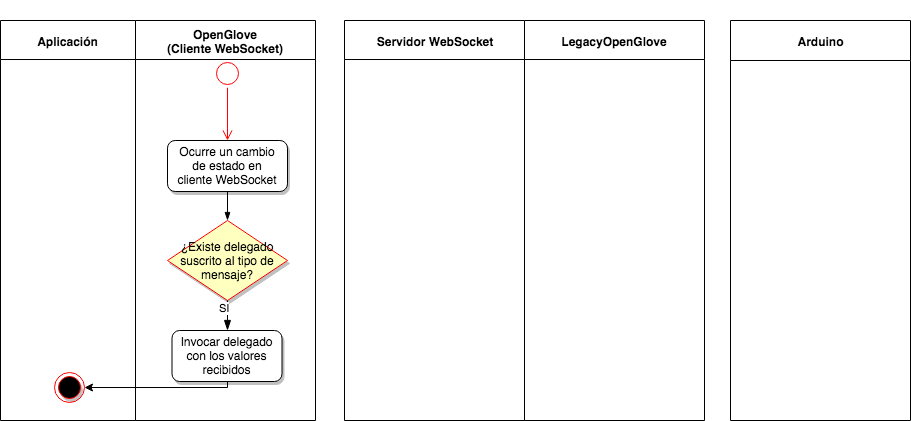
\includegraphics[width=1.0\textwidth]{images/chapter04/ActivityDiagrams-ListeningFromWebSocketClient.png} 
   	\captionsetup{justification=centering}
    \caption[Diagrama de actividades del método que escucha la conexión del dispositivo Bluetooth]{Diagrama de actividades del método que escucha la conexión del dispositivo Bluetooth\\Fuente: Elaboración propia (2018)}
    \label{fig:activity-diagrams-6-listening-websocket-state}
  \end{center}
\end{figure}